\section*{Preliminaries} \label{prel:vari}

As previously mentioned, in 2017 Muggli et al.~\cite{vari} presented $\vari$, which is a representation of the colored de Bruijn graph using BWT.  Our proposed method, $\ours$, efficiently merges de Bruijn graphs that are represented in this manner. Therefore, we first define some basic notation and definitions concerning BWT, then we show how the de Bruijn graph can be stored using BWT, and finally, we show how the {\em colored} de Bruijn graph can be stored succinctly.  We refer the reader to the full paper by Muggli et al.~\cite{vari} for a more detailed discussion of the representation.   

\subsection*{Basic Definitions and Terminology} %\subsection{sec:basic}

Here, we begin with some basic definitions related to our representation.  Throughout we consider a string $\X = \X[1..n] = \X[1]\X[2]\ldots
\X[n]$ of $|\X| = n$ symbols drawn from the alphabet $[0..\sigma-1]$.
%We assume $\X[n]$ is a special ``end of string'' symbol, \$, smaller than
%all other symbols in the alphabet.
For $i=1,\ldots,n$ we
write $\X[i..n]$ to denote the {\em suffix} of $\X$ of length $n-i+1$,
that is $\X[i..n] = \X[i]\X[i+1]\ldots \X[n]$.  
%We will often refer to suffix $\X[i..n]$ simply as ``suffix $i$''. 
Similarly, we write
$\X[1..i]$ to denote the {\em prefix} of $\X$ of length $i$.
$\X[i..j]$ is the {\em substring} $\X[i]\X[i+1]\ldots \X[j]$ of $\X$
that starts at position $i$ and ends at $j$. 
%By $\X[i..j)$ we
%denote $\X[i..j-1]$.  If $j < i$ we
%define $\X[i..j]$ to be the empty string, also denoted by
%$\varepsilon$.

\paragraph*{Suffix arrays and suffix array intervals.}
The suffix array~\cite{mm1993} $\SA_{\X}$ (we drop subscripts when
they are clear
from the context) of a string $\X$
is an array $\SA[1..n]$ which
contains a permutation of the integers $[1..n]$ such that $\X[\SA[1]..n]
\prec \X[\SA[2]..n] \prec \cdots \prec \X[\SA[n]..n]$.  In other words, $\SA[j] =
i$ if and only if $\X[i..n]$ is the $j^{\mbox{{\scriptsize th}}}$ suffix of $\X$
in lexicographical order. Here, $\prec$ denotes lexicographic precedence.

%The inverse
%suffix array $\ISA$ is the inverse permutation of $\SA$, that is
%$\ISA[i] = j$ iff $\SA[j] = i$.
%Conceptually, $\ISA[i]$ tells us the position of suffix $i$ in $\SA$. 

%Our data structure for colored de Bruijn graphs is based on a succinct representation of individual de Bruijn graphs that was introduced by Bowe et al.~\cite{BOSS12} and which we refer to as the BOSS representation from the authors' initials.  The BOSS representation was in turn based on an adaptation of Ferragina and Manzini's~\cite{FM05} FM-indexes.  Before getting to our description of the succinct colored de Bruijn graph data structure, 
%In the rest of this section 
%we first describe FM-indexes and then explain the BOSS representation.Our explanation of BOSS is particularly simple and may be of independent interest to those wanting to better understand that data structure.
% This new take on BOSS was key to our development of our succinct colored de Bruijn graph. 
% Travis: No it wasn't, it came afterward. :o)

For a string $\Y$, the $\Y$-interval in the suffix array $\SA_{\X}$ is
the interval $\SA[s..e]$ that contains all suffixes having $\Y$ as a
prefix. The $\Y$-interval is a representation of the occurrences of
$\Y$ in $\X$. For a character $c$ and a string $\Y$, the computation
of $c\Y$-interval from $\Y$-interval is called a \emph{left extension}.
%and the computation of $\Y$-interval from ${\Y}c$-interval is called a
%\emph{right contraction}. \emph{Left contraction} and \emph{right
%  extension} are defined symmetrically.

\paragraph*{BWT.} Next, for a string $\Y$, let $\F$ be the list of $\Y$'s characters sorted lexicographically by the suffixes starting at those characters, and $\L$ be the list of $\Y$'s characters sorted lexicographically by the suffixes starting immediately after those characters.  (The names $\F$ and $\L$ are standard for these lists.)  If \(\Y [i]\) is in position $p$ in $\F$ then \(\Y [i - 1]\) is in position $p$ in $\L$.  Moreover, if \(\Y [i] = \Y [j]\) then \(\Y [i]\) and \(\Y [j]\) have the same relative order in both lists; otherwise, their relative order in $\F$ is the same as their lexicographic order.  This means that if \(\Y [i]\) is in position $p$ in $\L$ then (assuming arrays are indexed from 0) in $\F$ it is in position
\[|\{h\,:\,\Y [h] \prec \Y[i]\}| + |\{h\,:\, \L [h] = \Y [i],\ h \leq p\}| - 1\,.\] Finally, notice that the last character in $\Y$ always appears first in $\L$.  It follows that we can recover $\Y$ from $\L$, which is the famous {\em Burrows-Wheeler Transform (BWT)}~\cite{bw1994} of $\Y$.


\paragraph*{FM-index and backward seach.}  Ferragina and Manzini~\cite{fm2005} first  realized BWT can be used for indexing in addition to compression.   Hence, if we know the range \(\BWT (\Y) [i..j]\) occupied by characters immediately preceding occurrences of a pattern $P$ in $\Y$, then we can compute the range \(\BWT (\Y) [i'..j']\) occupied by characters immediately preceding occurrences of \(c P\) in $\Y$, for any character $c$, since
\begin{eqnarray*}
i' & = & |\{h\,:\,\Y [h] \prec c\}| + |\{h\,:\,\Y [h] = c, h < i\}| \\
j' & =  & |\{h\,:\,\Y [h] \prec c\}| + |\{h\,:\, \Y [h] = c, h \leq j\}| - 1\,.
\end{eqnarray*}
Notice \(j' - i' + 1\) is the number of occurrences of \(c P\) in $S$.  The essential components of an FM-index for $\Y$ are: (1) an array storing \(|\{h\,:\,\Y [h] \prec c\}|\) for each character $c$ and, (2) a {\em rank} data structure for \(\BWT (\Y)\) that quickly tells us how often any given character occurs up to any given position. To be able to locate the occurrences of patterns in $\Y$ (in addition to just counting them), we can use a sampled suffix array of $\Y$ and a bitvector indicating the positions in \(\BWT (\Y)\) of the characters preceding the sampled suffixes.  

Hence, we define the function
$\rank(\Y, c,i)$, for string $\Y$, symbol $c$, and integer $i$, as 
the number of occurrences of $c$ in $\Y[1..i]$. Rank is used in {\em backward search}~\cite{fm2005} in order to compute left extension of a given string, i.e., the previous character. 

 %  It is well known that $\LF[i] = \C[\BWT[i]] + \rank(\BWT,\BWT[i],i)$.  Furthermore, we can compute the left extension using $\C$ and $\rank$.  If $\SA[s..e]$ is the $\Y$-interval,
%containing all the suffixes prefixed with string $\Y$,  then $\SA[\C[c]+\rank(\BWT,c,s),\C[c]+\rank(\BWT,c,e)]$ is the $c\Y$-interval. This is called \emph{backward search}~\cite{fm2005}, and a data structure supporting it is called an {\em FM-index}.


\subsection*{Storage of de Bruijn Graph using BWT} 

Given a de Bruijn graph $G =(V, E)$, we refer to the label of an edge $e \in E$ as the $k$-mer corresponding to it, and denote it as $\elabel(e)$.  Further, given $V$, we define the co-lexicographic (colex) ordering of $V$ as the lexicographic order of their reversed labels ($(k - 1)$-mers).  

We let $\F$ be the edges in $E$ in colex order by their ending nodes, where ties are broken by their starting nodes, and let $\L$ be the edges in $E$ sorted colex by their starting nodes, with ties broken by their ending nodes.  We refer to the ordering of $\L$ as {\em Vari-sorted}. If we are given two edges $e$ and $e'$ that have the same label then we are guaranteed that they have the same relative order in both $\F$ and $\L$; otherwise, their relative order in $\F$ is the same as their labels' lexicographic order.  This means that if $e$ is in position $p$ in $\L$, then in $\F$ it is in position
\[|\{d\,:\,d \in E,\ \elabel (d) \prec \elabel (e)\}| + \]
	\[ |\{h\,:\,\elabel (\L [h]) = \elabel (e),\ h \leq p\}| - 1\,\]
where $\prec$ denotes lexicographic precedence.  We define the edge-$\BWT$ ($\EBWT$) of $G$ to be the sequence of edge labels sorted according to the ordering of the edges in $\L$, so \(\elabel (\L [h]) = \EBWT (G) [h]\) for all $h$. Therefore, if we have an array $D$ storing \(|\{d\,:\,d \in E,\ \elabel (d) \prec c\}|\) for each character $c$ and  a fast rank data structure on \(\EBWT (G)\) then given an edge's position in $\L$, we can quickly compute its position in $\F$.

We let $\B_F$ be the bit vector with a 1 marking the position in $\F$ of the last incoming edge of each node, and let $\B_L$ be the bit vector with a 1 marking the position in $\L$ of the last outgoing edge of each node.  Given a character $c$ and the colex rank of a node $v$, we can use $\B_L$ to find the interval in $\L$ containing $v$'s outgoing edges.  We can then search \(\EBWT (G)\) to find the position of each outgoing edge\footnote{In practice, we incorporate the bits of $B_F$ as flags on \(\EBWT (G)\) and use them to obtain the colex order of $v$ but omit the discussion here for simplicity.  We refer the reader to Bowe et al.~\cite{BOSS} for a full discussion of this aspect and the supplement for our handling here.}. Similarly, we can make similar queries about the incoming edges of a node $v$ in an efficient manner using $\B_F$.  

%In addition, if $B_G$ is  the bit vector with a 0 marking the position in $\F$ of the first incoming edge of each node, we define $\flags$ to be the vector that stores the permutation from $\F$ to $\L$ applied to $\B_G$.  Next, we see how we use $\flags$.  If we are given a character $c$ and the colex rank of a node $v$, we can use $\B_L$ to find the interval in $\L$ containing $v$'s outgoing edges, then we can search in \(\EBWT (G)\) to find the position of the one $e$ labeled $c$.  We need $\flags$ in order to obtain the colex rank of $v$.  Thus, we can find $e$'s position in $\F$, as described above.  Finally, we can use $\B_F$ to find the co-lexicographic rank of $e$'s ending node.  

Therefore, briefly we explained how we can construct and represent a de Bruijn graph $G = (V, E)$ with $\EBWT$, $\B_L$,  and $\B_F$ in a manner that allows for efficient navigation of the graph. An example of this representation is shown in Figure \ref{fig:purple}. Given this representation we can traverse the graph and recover incoming and outgoing edges.   Next, we demonstrate how the labels ($k$-mers) can be recovered using this data structure.

%With the appropriate implementations of the data structures, we obtain the following result:
%\begin{theorem}[Bowe, Onodera, Sadakane and Shibuya, 2012]
%We can store $G$ in \((1 + o (1)) |E| (\lg \sigma + 2)\) bits such that, given a character $c$ and the co-%lexicographic rank of a node $v$, in $O{\log \log \sigma}$ time we can find the node reached from $v$ by following the directed edge labelled $c$, if such an edge exists.
%\end{theorem}

\paragraph*{Label recovery.}  We note that an important aspect of this succinct representation of the graph is that the $(k - 1)$-mers (nodes) and $k$-mers (edges) of the de Bruijn graph $G$ are not explicitly stored in the above representation---rather they than can be {\em computed} (or recovered) from this representation.    As previously mentioned, we can traverse the graph in a forward or reverse manner and recover incoming and outgoing edges of a given node $v$.  Given this efficient traversal, we can recover the label of $v$ by traversing the graph in a backward direction starting from $v$;  given the label of $v$ is a $(k - 1)$-mer we traverse backward $k - 1$ times.  Therefore, we must add extra nodes and edges to the graph to ensure there is a directed path of length at least \(k - 1\) to each original node.  More formally, we augment the graph so that each new node's label is a \((k - 1)\)-mer that is prefixed by one or more copies of a special symbol $\$$ not in the alphabet and lexicographically strictly less than all others.  When new nodes are added, we are assured that the node labeled $\$^{k - 1}$ is always first in colex order and has no incoming edges.  Lastly, we augment the graph in a similar manner by adding an extra outgoing edge, labeled $\$$, to each node with no outgoing edge.   These ``dummy nodes'' are shown in Figure \ref{fig:purple}.


%Here, we briefly describe the procedure for recovering these node and edge labels.  This method could be used for a trivial merge algorithm that we will discuss later.  

%If we know the range \(\B_L [i..j]\) of $k$-mers whose starting nodes end with a pattern $P$ of length less than \((k - 1)\), then we can compute the range \(\B_F [i'..j']\) of $k$-mers whose ending nodes end with \(P c\), for any character $c$, since
%\begin{eqnarray*}
%i' & = & |\{d\,:\,d \in E,\ \elabel (d) \prec c\}|  \\
 %  & & + |\{h\,:\,\EBWT (G) [h] = c,\ h < i\}|\\
%j' & = & |\{d\,:\,d \in E,\ \elabel (d) \prec c\}| \\
% &  & + |\{h\,:\,\EBWT (G) [h] = c,\ h \leq j\}| - 1\,.
%\end{eqnarray*}

%^Thus,  we can find the interval in $\B_L$ containing $v$'s outgoing edges in $O(k \log \log \sigma)$-time, provided there is a directed path to $v$ of length at least \(k - 1\) but note that we cannot use \(\EBWT (G)\), $\B_F$ and $\B_L$ alone to recover the labels of nodes with no incoming edges.  Thus, we add extra nodes and edges to the graph to ensure there is a directed path of length at least \(k - 1\) to each original node.  More formally, we augment the graph so that each new node's label is a \((k - 1)\)-mer that is prefixed by one or more copies of a special symbol $\$$ not in the alphabet and lexicographically strictly less than all others.  When new nodes are added, we are assured that the node labeled $\$^{k - 1}$ is always first in colex order and has no incoming edges.  Lastly, we augment the graph in a similar manner by adding an extra outgoing edge, labeled $\$$, to each node with no outgoing edge.  

\subsection*{Storage of Colors} 

Given a multiset \(\mathcal{G} = \{G_1, \ldots, G_t\}\) of individual de Bruijn graphs, we set $G$ to be the union of those individual graphs and build the previously described representation for $G$.  We also build and store a two-dimensional binary array $\C$ in which \(\C [i, j]\) indicates whether the $i$th edge in $G$ is present in the $j$th individual de Bruijn graph (i.e., whether that edge has the $j$th color).    Hence, we store a given de Bruijn graph using $\EBWT$, the described bit vectors, and a compressed color matrix.  The combination of the above storage of the graph $G$ plus the compressed matrix is the succinct storage of the graph. 



\begin{figure}
\centering
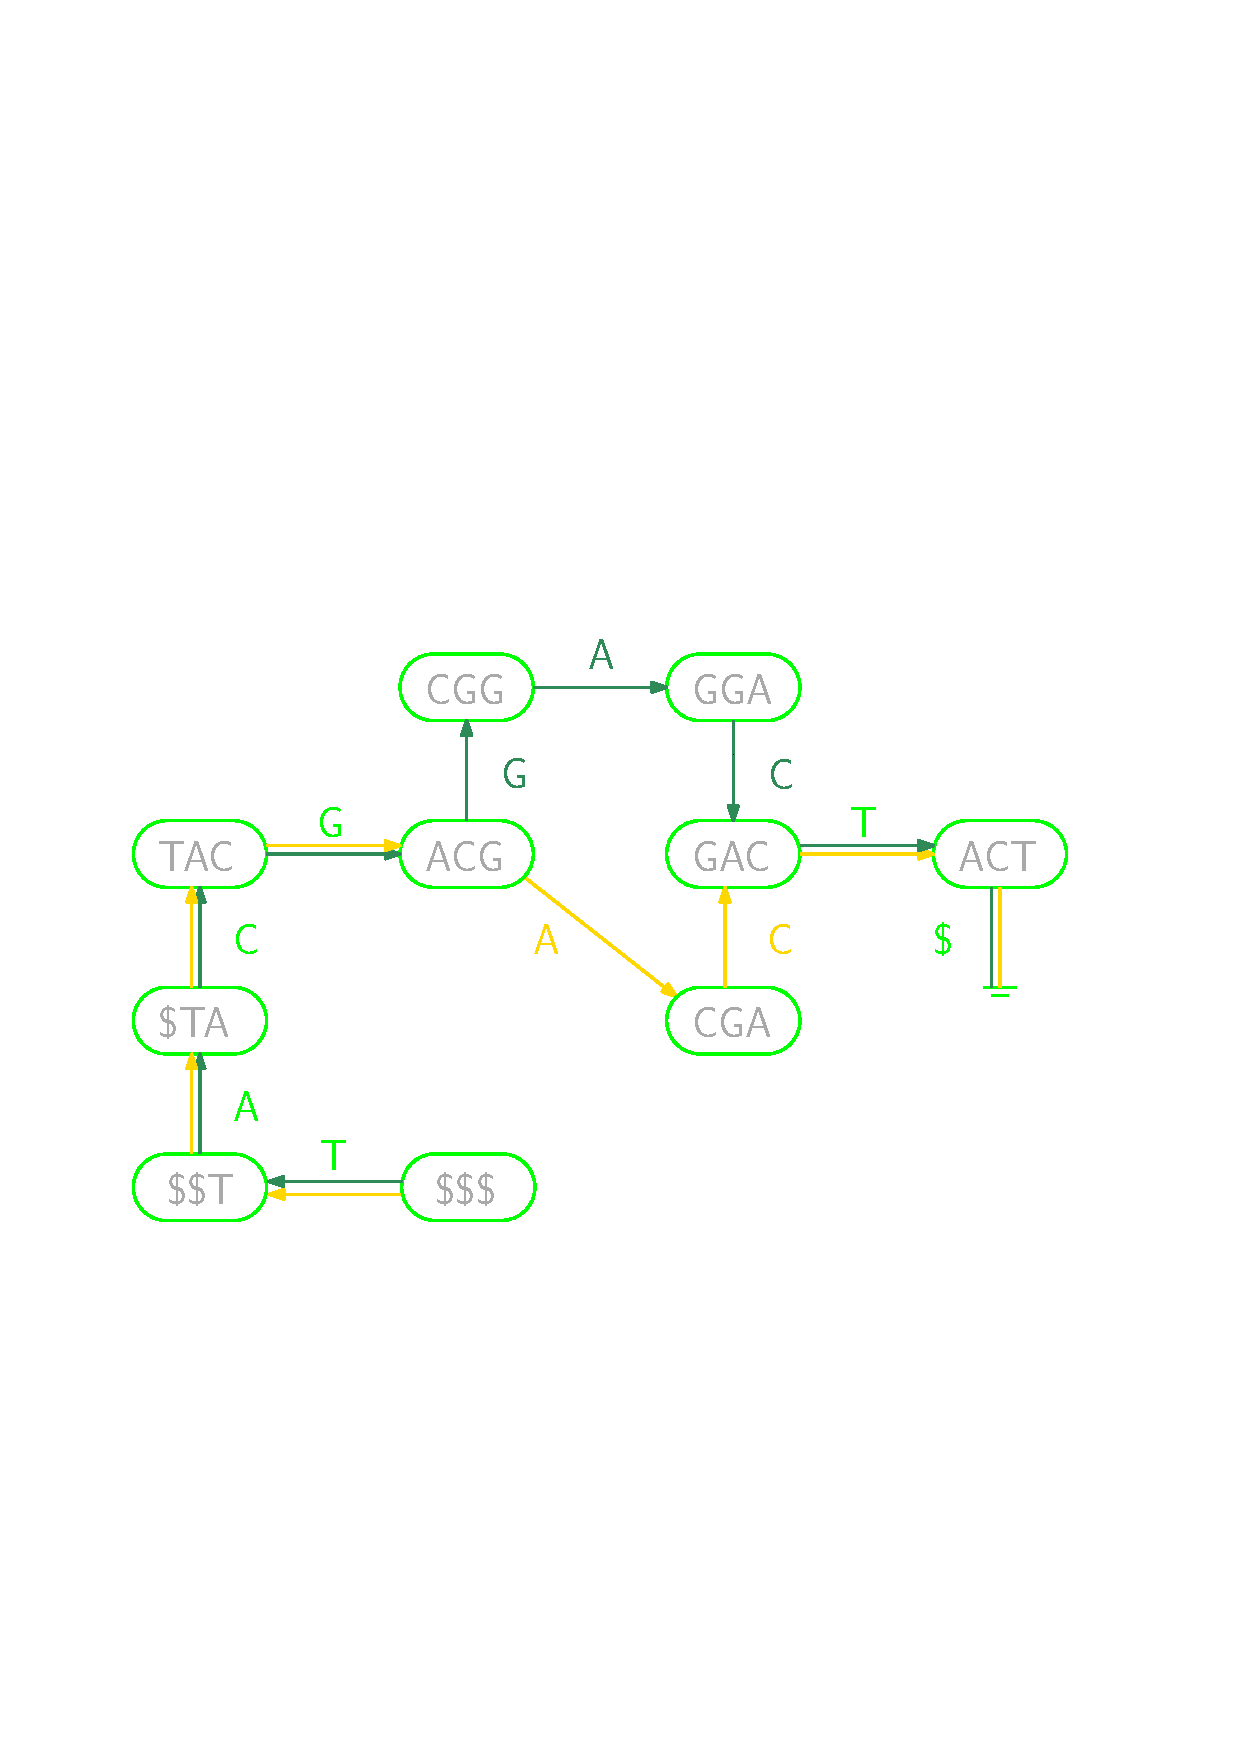
\includegraphics[width=.35\textwidth]{limegraph.pdf} \\~\\
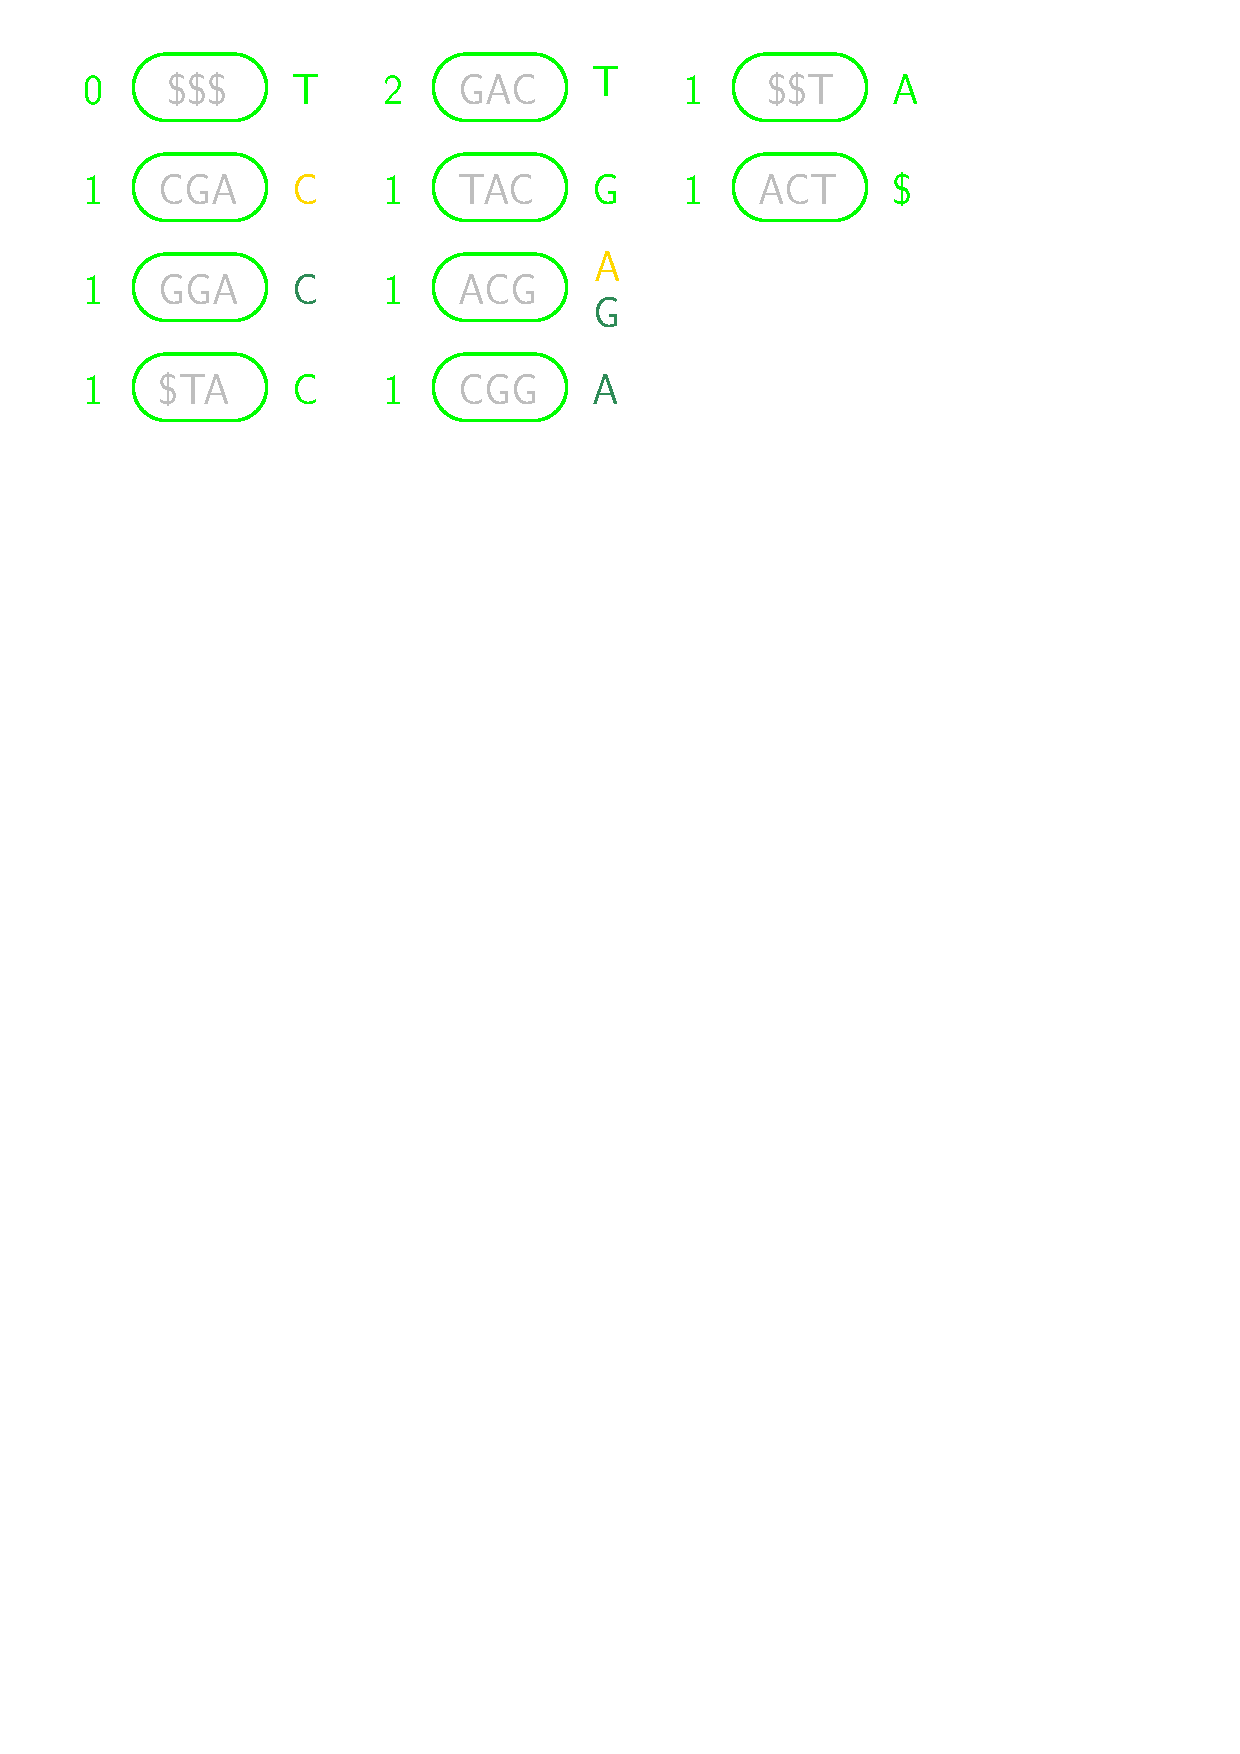
\includegraphics[width=.35\textwidth]{limeonlymapping.pdf} \\~\\
\raisebox{0.1ex}{$\begin{array}{rr}
   \EBWT (G) = &  \mathtt{TCCCTGAGAA\$}\\[1ex]
         \B_F = & \mathtt{ 1110111111}\\
         \B_L = & \mathtt{11111101111}\\[1ex]
C^\mathrm{T} = &   \mathtt{11011110011}\\
               &  \mathtt{10111101111}
\end{array}$}
%\end{tabular}
\caption{{\bf Top:} A colored de Bruijn graph consisting of two individual graphs, whose edges are shown in yellow and green. All nodes to be present in both graphs are shown in lime.  {\bf Below:} The $\vari$ representation of the colored de Bruijn graph: the edge-BWT and bitvectors for the union of the individual graphs, and the binary array $C$ (shown transposed) whose bits indicate which edges are present in which individual graphs.}
\label{fig:purple}
\end{figure}
